\documentclass[12pt,a4paper]{report}

\usepackage[utf8]{inputenc}
\usepackage[T1]{fontenc}
\usepackage[top=1in,bottom=1in,left=1.28in,right=0.98in]{geometry}
\usepackage{times}
\usepackage{graphicx}
\usepackage{float}
\usepackage{titlesec}
\usepackage{fancyhdr}
\usepackage{enumitem}
\usepackage{caption}
\usepackage{chngcntr}
\usepackage{setspace}
\usepackage[hidelinks]{hyperref}

\onehalfspacing
\counterwithin{figure}{chapter}
\counterwithin{table}{chapter}

\captionsetup[figure]{labelfont=it,textfont=it,labelsep=space,name={Fig no},labelformat=simple}
\captionsetup[table]{labelfont=it,textfont=it,labelsep=space,name={Table},labelformat=simple}

% Chapter heading: "CHAPTER 1: INTRODUCTION" centred, bold, one line
\titleformat{\chapter}[block]
  {\centering\normalfont\bfseries\LARGE}
  {CHAPTER \thechapter:}
  {0.5em}
  {\MakeUppercase}
\titlespacing*{\chapter}{0pt}{0pt}{30pt}

% Body page header/footer
\fancypagestyle{bodyps}{
  \fancyhf{}
  \fancyhead[L]{\textit{Minor Miniproject Report}}
  \fancyfoot[L]{\textit{Dept. of ER, SJCET, Palai}}
  \fancyfoot[R]{\textit{Page \thepage}}
  \renewcommand{\headrulewidth}{0.4pt}
  \renewcommand{\footrulewidth}{0.4pt}
}
% Front-matter page style: centred page number only, no rules
\fancypagestyle{frontps}{
  \fancyhf{}
  \fancyfoot[C]{\thepage}
  \renewcommand{\headrulewidth}{0pt}
  \renewcommand{\footrulewidth}{0pt}
}

\newcommand{\TITLE}{AI-BASED PREDICTIVE BLIND-SPOT MONITORING AND INTELLIGENT HUMAN SAFETY ANALYSIS SYSTEM FOR VEHICLES}

\begin{document}

% ======================================================================
% COVER PAGE
% ======================================================================
\thispagestyle{empty}
\begin{center}
\vspace*{0.3in}
{\bfseries\large MINOR MINIPROJECT REPORT ON}\\[14pt]
{\bfseries\large \TITLE}\\[18pt]

In partial fulfilment of the requirements for the award of the Minor degree of\\[8pt]
{\bfseries\large BACHELOR OF TECHNOLOGY}\\[4pt]
in\\[4pt]
{\bfseries\large ROBOTICS AND AUTOMATION}\\[24pt]

Submitted by\\[8pt]
{\bfseries ANUSREE ANIL (Reg. No: SJC23AD016)}\\[4pt]
{\bfseries DEVADARSAN C P (Reg. No: SJC23AD027)}\\[4pt]
{\bfseries GEORGY ANTONY PIOUS (Reg. No: SJC23AD035)}\\[4pt]
{\bfseries RINO ROBERT (Reg. No: SJC23AD064)}\\[24pt]


\includegraphics[width=1.1in]{images/college_logo.png}\\[14pt]

{\bfseries ST.\ JOSEPH'S COLLEGE OF ENGINEERING \& TECHNOLOGY (AUTONOMOUS)}\\[2pt]
{\bfseries CHOONDACHERRY P.O., PALAI -- 686579}\\[2pt]
{\bfseries DEPARTMENT OF ELECTRONICS \& COMPUTER ENGINEERING}\\[2pt]
{\bfseries NOVEMBER, 2026}
\end{center}
\newpage

% ======================================================================
% CERTIFICATE
% ======================================================================
\thispagestyle{empty}
\begin{center}
{\bfseries ST.\ JOSEPH'S COLLEGE OF ENGINEERING \& TECHNOLOGY PALAI (AUTONOMOUS)}\\[2pt]
{\bfseries DEPARTMENT OF ELECTRONICS \& COMPUTER ENGINEERING}\\[2pt]
CHOONDACHERRY P.O., PALAI -- 686579\\[2pt]
\textit{(An ISO 9001:2015 Certified Institution)}\\[20pt]
{\bfseries\Large Certificate}
\end{center}
\vspace{10pt}

\noindent This is to certify that the course project report entitled \textquotedblleft\TITLE\textquotedblright\ is the bonafide work of Ms.\ Anusree Anil (Reg.\ No.\ SJC23AD016), Mr.\ Devadarsan C P (Reg.\ No.\ SJC23AD027), Mr.\ Georgy Antony Pious (Reg.\ No.\ SJC23AD035) and Mr.\ Rino Robert (Reg.\ No.\ SJC23AD064) to the Department of Electronics \& Computer Engineering, St.\ Joseph's College of Engineering \& Technology, Palai, in partial fulfilment of the requirements for the Minor Degree of Bachelor of Technology in Robotics \& Automation from APJ Abdul Kalam Technological University, Kerala, carried out under our supervision and guidance.

\vspace{8pt}
\noindent We hereby certify that the work reported in this project is original and has been carried out by the students mentioned above under our supervision.

\vspace{20pt}
\noindent Place: Palai \hfill Date: \underline{\hspace{1.2in}}

\vspace{30pt}
\noindent
\begin{minipage}[t]{0.58\textwidth}
{\bfseries Ms.\ Soya Tressa Jose}\\
Asst.\ Professor, Dept.\ ER\\[10pt]
{\bfseries Fr.\ Dan Thankachan}\\
Asst.\ Professor, Dept.\ ER\\
Project Coordinators
\end{minipage}%
\begin{minipage}[t]{0.38\textwidth}
{\bfseries Dr.\ Giby Jose}\\
HoD -- ER
\end{minipage}
\newpage

% ======================================================================
% FRONT MATTER (roman numerals)
% ======================================================================
\pagenumbering{roman}
\setcounter{page}{1}
\pagestyle{frontps}

\chapter*{ACKNOWLEDGEMENT}
\addcontentsline{toc}{chapter}{ACKNOWLEDGEMENT}

First and foremost, we thank God Almighty for giving us the inner strength, resources, and ability to complete this work successfully, without which all our efforts would have been in vain.

We are grateful to Dr.\ Giby Jose, Head of the Department of Electronics \& Computer Engineering, for his valuable advice and motivation throughout the course of our project.

We sincerely thank our Mini Project Coordinators, Ms.\ Soya Tressa Jose and Fr.\ Dan Thankachan (Assistant Professors, Department of Electronics \& Computer Engineering), for their constant guidance, valuable advice, and support during the project.

We also convey our sincere thanks to Ms.\ Christy Joy, our project guide (Assistant Professor, Department of Electronics \& Computer Engineering), for her encouragement and assistance throughout this project.

Finally, we express our heartfelt gratitude to our parents and friends for their continuous support, and to all those who have directly or indirectly contributed to the successful completion of this project.
\newpage

\chapter*{ABSTRACT}
\addcontentsline{toc}{chapter}{ABSTRACT}

Vehicle blind spots pose a persistent safety challenge, as pedestrians and other people may enter regions that are not clearly visible to the driver. Basic human detection alone offers limited insight, since it does not indicate how a person is moving or whether their path may lead towards a hazardous area. This project proposes an AI-based, vision-driven vehicle safety monitoring system that goes beyond simple detection by combining persistent tracking, movement analysis and predictive risk assessment. Humans are detected in video frames using YOLOv8, and ByteTrack assigns each person a unique identity that is maintained across consecutive frames. Movement direction analysis interprets how each tracked individual is moving, and short-term trajectory prediction estimates their likely future positions. Vehicle blind-spot regions are represented as configurable polygon-based danger zones that can be adapted to different camera views. The predictive risk assessment module identifies potential conflicts between predicted trajectories and these zones, and generates explainable safety alerts that state the reasons behind each identified risk. These alerts are advisory safety warnings intended to support the driver. A Streamlit dashboard displays the processed video, tracking information, alerts and event statistics, while event logging maintains safety-related records for later analysis. Webcams and prerecorded video footage are used for software demonstrations, testing and simulation, and vehicle-mounted wide-angle cameras are envisioned for future real-world deployment. By integrating detection, tracking, trajectory prediction and risk assessment, the proposed system is expected to improve driver awareness and support intelligent vehicle safety monitoring. Since predictions are short-term estimates, the system is intended as a decision-support aid and not as a substitute for driver attention.
\newpage

\tableofcontents
\newpage
\listoffigures
\listoftables
\newpage

\chapter*{LIST OF ABBREVIATIONS}
\addcontentsline{toc}{chapter}{LIST OF ABBREVIATIONS}
\begin{center}
\begin{tabular}{|p{1.6in}|p{4.3in}|}
\hline
\textbf{Abbreviation} & \textbf{Expansion} \\ \hline
AI & Artificial Intelligence \\ \hline
API & Application Programming Interface \\ \hline
CNN & Convolutional Neural Network \\ \hline
CPU & Central Processing Unit \\ \hline
FPS & Frames Per Second \\ \hline
GPU & Graphics Processing Unit \\ \hline
GUI & Graphical User Interface \\ \hline
ID & Identifier \\ \hline
IoU & Intersection over Union \\ \hline
ML & Machine Learning \\ \hline
ROI & Region of Interest \\ \hline
SDG & Sustainable Development Goal \\ \hline
SQL & Structured Query Language \\ \hline
UI & User Interface \\ \hline
UN & United Nations \\ \hline
YOLO & You Only Look Once \\ \hline
\end{tabular}
\end{center}
\newpage

% ======================================================================
% BODY (arabic numerals)
% ======================================================================
\pagenumbering{arabic}
\setcounter{page}{1}
\pagestyle{bodyps}

\chapter{INTRODUCTION}

\section{Overview}
Large vehicles such as buses have significant blind-spot regions around their front, rear and sides, where pedestrians and other road users may be present without being visible to the driver. News reports continue to highlight the real-world consequences of this gap: a school-bus accident reported by Asianet News on 20 November 2025, and a woman struck by a school bus, reportedly in the driver's blind spot, reported by the Times of India on 24 February 2025, illustrate the continuing need for better blind-spot awareness systems.

This project, AI-Based Predictive Blind-Spot Monitoring and Intelligent Human Safety Analysis System for Vehicles, is a software-only vision system that goes beyond simple human detection. It combines YOLOv8-based detection, persistent multi-person tracking with ByteTrack, movement-direction analysis, short-term trajectory prediction and a rule-based, explainable risk-assessment engine to identify people who are already inside, or are likely to soon enter, a configurable danger zone around the vehicle, and to raise advisory safety alerts for the driver.

\section{Problem Identification}
The problem was identified by reviewing existing blind-spot and pedestrian-detection systems and relevant literature. The following observations were made:
\begin{itemize}[leftmargin=*,itemsep=2pt]
\item Conventional human-detection-only systems indicate that a person is present but not how they are moving or whether their path is likely to lead into a hazardous area.
\item Basic proximity- or zone-based warning systems assess risk only from the current position of a person, without considering their direction of movement or likely future position.
\item Detection without persistent identity means the same person can be counted or logged multiple times across frames, and no movement history can be built up for them.
\item Existing simple systems provide little or no explanation for why an alert was raised, and keep no structured history of safety-relevant events for later review.
\end{itemize}
From these observations, a clear gap was identified: there is a need for a vision-based system that tracks people persistently, analyses their movement, predicts likely near-term danger-zone entries, and explains its own alerts.

\section{Social Relevance and Need}
Pedestrian safety around large vehicles, particularly buses used for school and public transport, is a matter of direct public concern, as reflected in recent news coverage of blind-spot-related accidents. The need for the proposed system can be summarised as follows:
\begin{itemize}[leftmargin=*,itemsep=2pt]
\item Target users: bus and large-vehicle drivers and transport operators, and researchers/students working on vehicle safety systems.
\item Safety impact: earlier and better-informed awareness of people in or approaching a vehicle's blind spot can reduce the risk of pedestrian--vehicle conflicts.
\item Accessibility impact: a software-only design that runs on an ordinary camera and laptop/embedded computer, without specialised sensors, keeps the approach accessible for retrofitting onto existing vehicles.
\end{itemize}

\section{Problem Formulation and Existing Solutions}
Problem statement: Conventional human-detection-based blind-spot monitoring systems indicate that a person is present but do not track that person persistently, analyse their movement, or predict whether their path is likely to enter a dangerous zone, limiting the usefulness and timeliness of the safety warnings they can provide.

An earlier baseline version of this project performed YOLOv8-based human detection with bounding-box visualisation, basic predefined blind-spot zone monitoring, a simple proximity/zone-based risk classification, and audio warning generation through an OpenCV-based interface. Its main limitations were: frame-by-frame detection without persistent person identities; no analysis of movement direction; no estimation of future trajectory; a single, fixed danger zone; a basic risk classification based only on current zone occupancy; and no structured event history or analytics for later review.

There is therefore a need for a system that builds on this baseline by adding persistent tracking, movement and trajectory analysis, configurable multi-zone geometry, a richer and explainable risk-assessment engine, and event logging with analytics.

\section{Proposed Concept}
The proposed concept is a software-only, camera-based safety-monitoring pipeline that processes a live webcam feed or a prerecorded video. Humans are detected using YOLOv8 and assigned persistent identities using ByteTrack. Each tracked person's recent movement is analysed to classify their direction and to estimate a short-term future position through linear trajectory extrapolation. Vehicle blind-spot regions are represented as configurable polygon-based danger zones, and a rule-based risk-assessment engine combines current zone occupancy, movement direction and predicted zone entry into a risk level from SAFE to CRITICAL, with a plain-language explanation attached to every decision.

Safety-relevant events are logged for later review, and a Streamlit-based dashboard presents the live feed, per-person predictive detail, zone configuration, incident analytics and a scenario simulator for testing on recorded video. The system is intended for webcam and prerecorded-video based demonstration, testing and simulation at this stage, with vehicle-mounted wide-angle cameras envisioned for future real-world deployment.

\section{Objectives}
\begin{itemize}[leftmargin=*,itemsep=2pt]
\item To detect humans in camera footage using YOLOv8 and monitor predefined blind-spot regions.
\item To assign persistent identities to detected people across consecutive frames using ByteTrack.
\item To analyse the movement direction of tracked people and estimate their short-term future positions.
\item To represent vehicle blind-spot regions as configurable, polygon-based danger zones.
\item To identify potential conflicts between predicted trajectories and danger zones and assign an explainable, dynamic risk level.
\item To generate advisory safety alerts with clear reasons and to maintain a structured history of safety-relevant events for later review.
\item To present the system's live output, predictive detail, zone configuration and incident analytics through an interactive dashboard.
\end{itemize}

\section{Organisation of the Report}
Chapter 2 presents the system architecture and the software and hardware requirements. Chapter 3 describes the per-frame detection, tracking and risk-assessment algorithm, along with the measured performance metrics and the implementation plan. Chapter 4 presents the results obtained from the working prototype, with screenshots of the dashboard. Chapter 5 gives the conclusion, the key outcomes, the limitations and future scope, and the alignment of the project with the UN Sustainable Development Goals.

% ======================================================================
\chapter{BLOCK DIAGRAM / SYSTEM DIAGRAM}

\section{System Architecture}
The system is organised as a pipeline, shown in Fig no 2.1. Each incoming video frame, from a webcam or a prerecorded video, is passed through human detection, persistent tracking, movement and trajectory analysis, danger-zone checking and risk assessment, in that order, and the result is used to drive audio alerts, event logging and the live dashboard display. The architecture is described module by module in the following sections.

\begin{figure}[H]
\centering
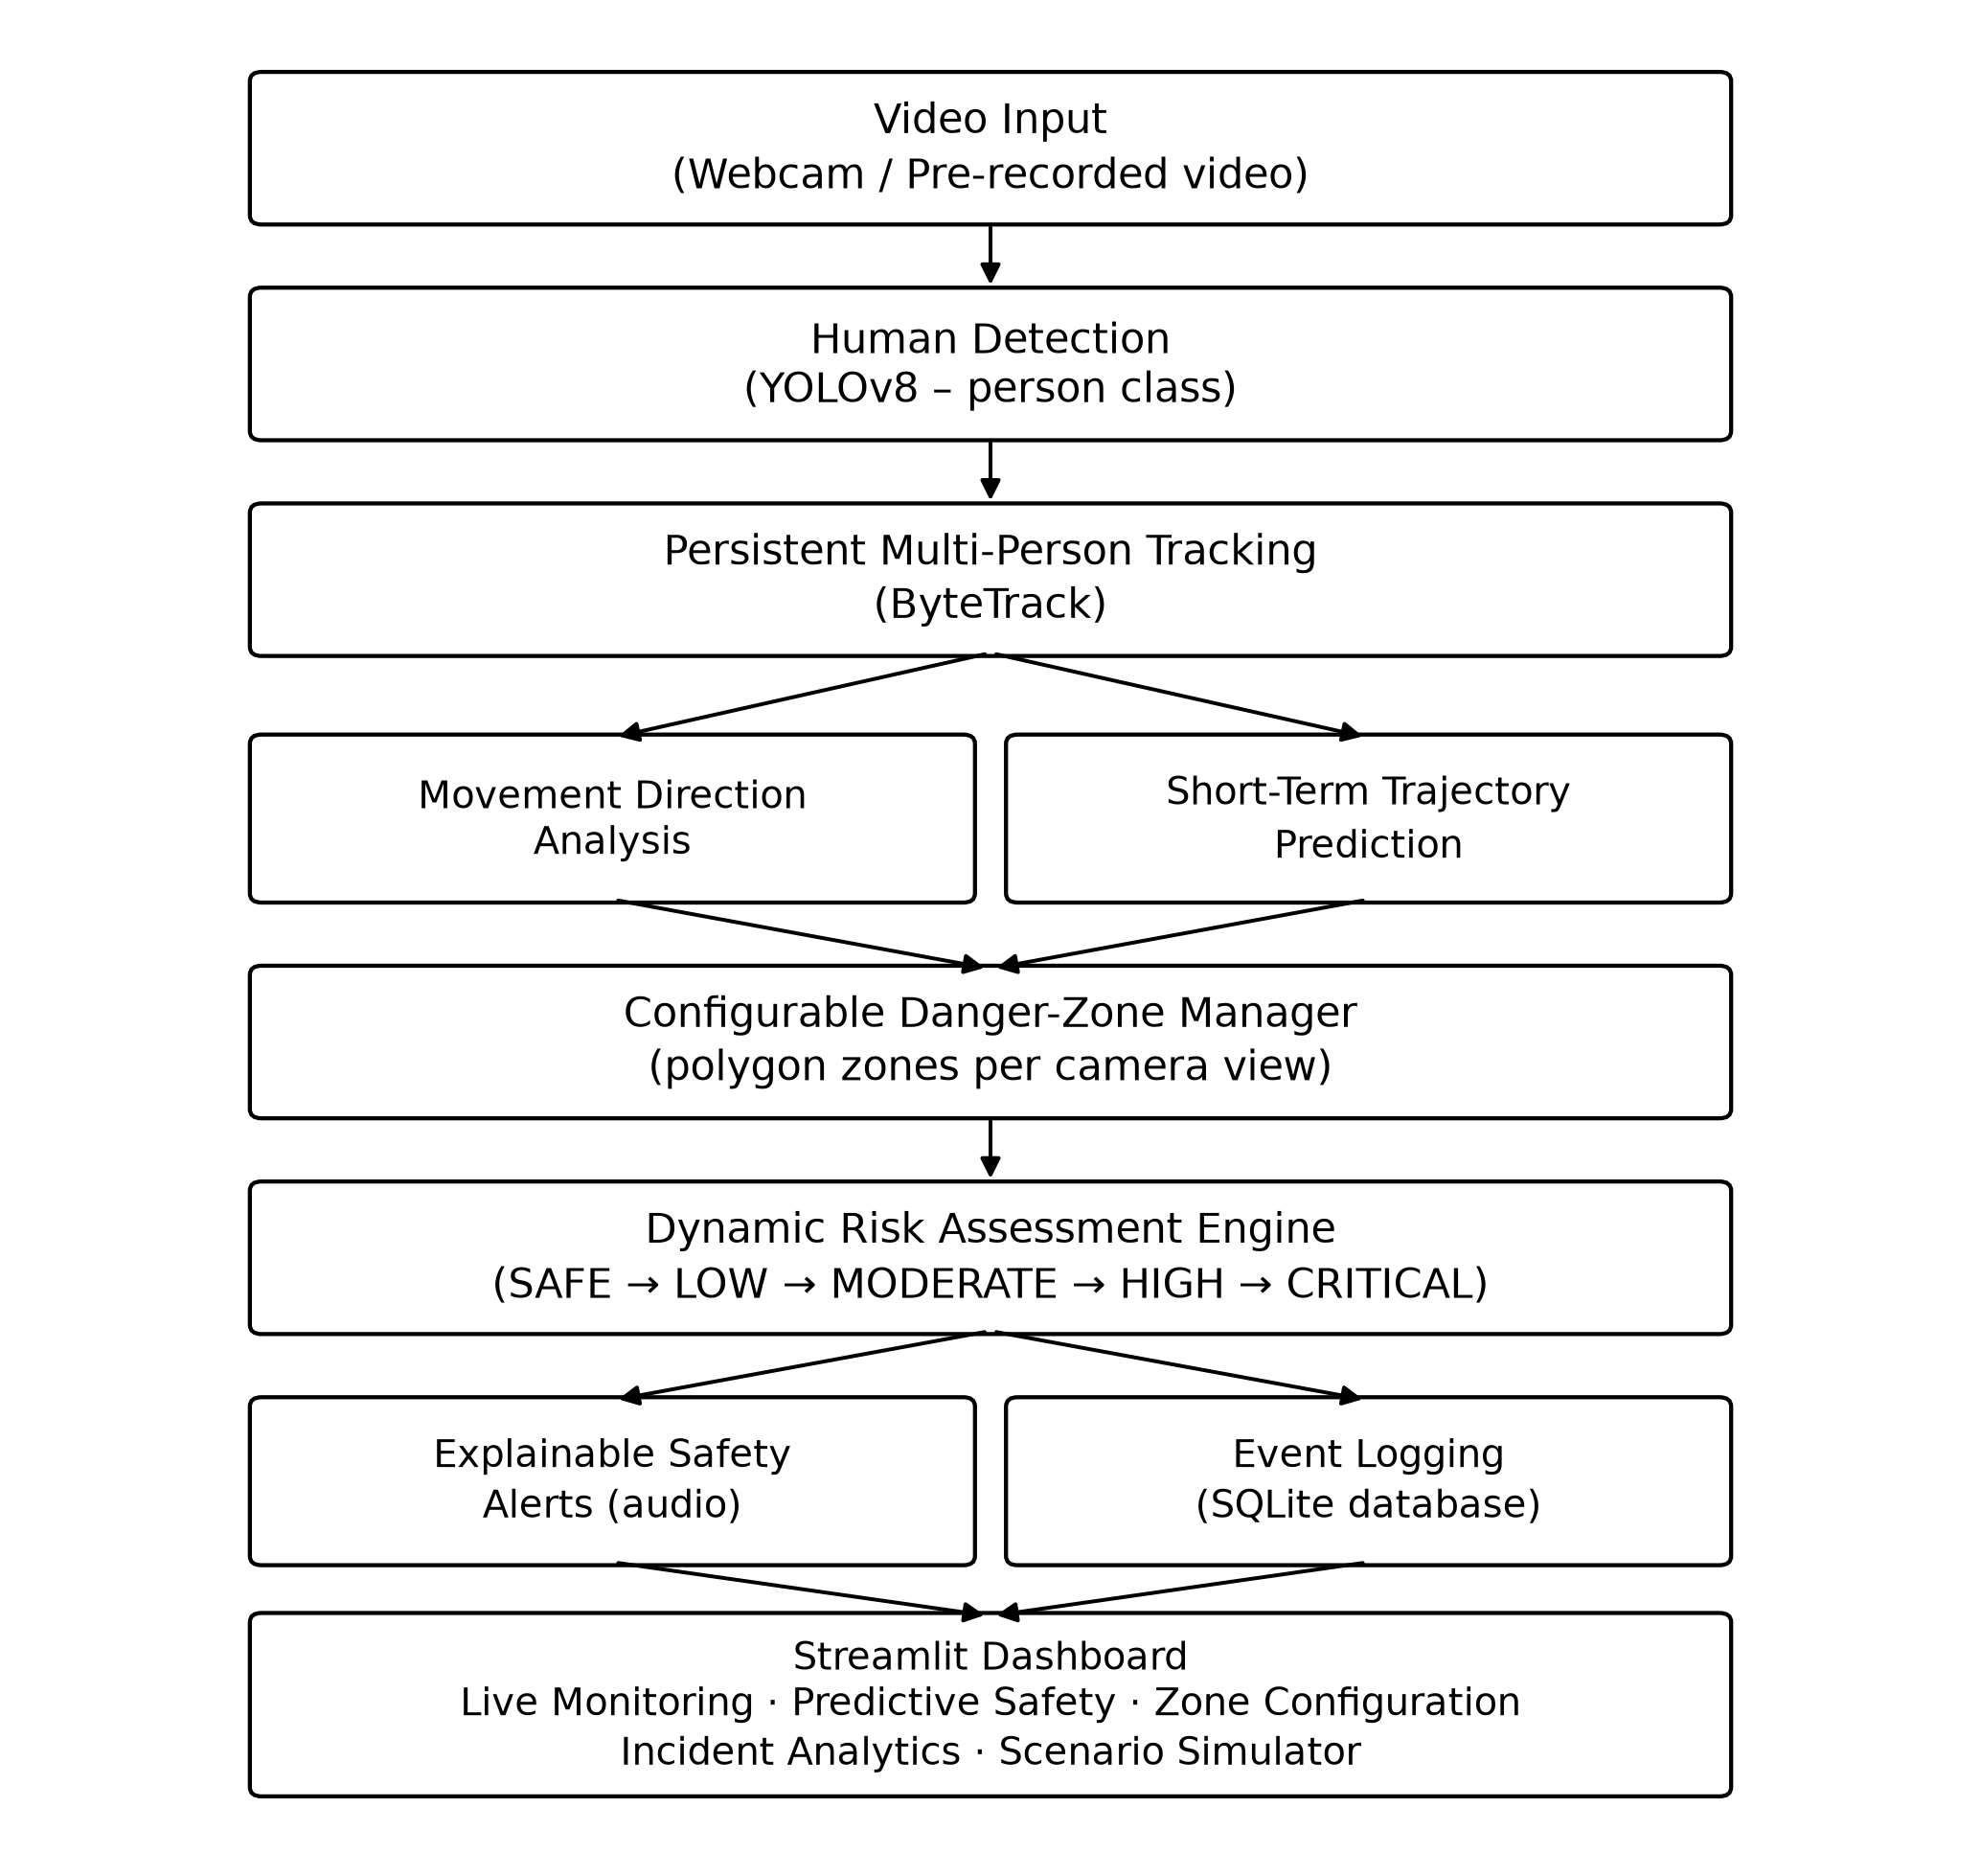
\includegraphics[width=5.6in]{images/fig_2_1_system_architecture.png}
\caption{System architecture of the blind-spot monitoring system}
\label{fig:2.1}
\end{figure}

\section{Human Detection and Tracking}
Each frame is processed by a YOLOv8n model restricted to the COCO ``person'' class, giving a bounding box and confidence score for every detected person. Ultralytics' built-in ByteTrack tracker is then used, through the model's own tracking mode with identity persistence enabled, to assign a stable tracking ID to each person and maintain that identity across consecutive frames, instead of treating every frame's detections as independent.

\section{Movement Direction Analysis and Trajectory Prediction}
For every tracked person, a short rolling history of recent positions and bounding-box sizes is maintained. This history is used, over a smoothing window of several frames, to classify the person's current movement as approaching, moving away, moving left, moving right, stationary, crossing, or unknown when there is not yet enough history. The same history is used by a simple linear extrapolation to estimate the person's likely position a short time ahead, and to check whether that projected position would fall inside an active danger zone before it actually happens, producing a predicted zone and an estimated time to entry.

\section{Configurable Danger-Zone Manager}
Blind-spot regions are represented as polygons, defined as fractions of the frame so that one definition works at any camera resolution, and grouped into named vehicle profiles, for example a bus profile with FRONT, LEFT, RIGHT and REAR zones. Each zone can be marked active or inactive; with a single camera, only the zone that camera actually observes is activated. For every tracked person, their position is tested against each active zone using a standard point-in-polygon test to determine current zone occupancy.

\section{Dynamic Risk Assessment and Explainability}
A rule-based risk engine combines current zone occupancy, movement direction and predicted zone entry into one of five risk levels, SAFE, LOW, MODERATE, HIGH or CRITICAL, with temporal hysteresis so that the risk level escalates immediately but only de-escalates after holding steady for several frames, avoiding frame-to-frame flicker. Every risk decision is accompanied by a plain-language explanation built directly from the same rule logic, for example stating that a person is inside a given zone and is getting closer to the camera, so that alerts are explainable rather than opaque.

\section{Alerting, Event Logging and Dashboard}
When the overall risk reaches HIGH or CRITICAL, a looping audio alert is triggered and a safety-relevant event is opened in a SQLite database; the same event is extended while the situation continues and closed once it clears, so that one continuous encounter is logged as a single event rather than one row per frame. A Streamlit-based dashboard presents the annotated live feed, a per-person predictive-safety panel, a visual zone-configuration editor, incident analytics computed from the logged events, and a scenario simulator for running the same pipeline over an uploaded or prerecorded test video.

\section{Software and Hardware Requirements}
\begin{itemize}[leftmargin=*,itemsep=2pt]
\item Software: Python 3.11+, the Ultralytics YOLOv8 implementation (with ByteTrack tracking), OpenCV, Streamlit for the dashboard, Plotly for analytics charts, and SQLite for event storage.
\item Hardware: a standard computer with a webcam; no specialised sensors, IoT devices or vehicle-mounted hardware are required for the current software-only implementation. A GPU is not required but improves the detection frame rate.
\end{itemize}

\section{Feasibility}
The system has been implemented and demonstrated end to end using standard, freely available software libraries on an ordinary laptop with a webcam, without any specialised hardware, confirming that the proposed approach is feasible within the project's resources and timeline.

% ======================================================================
\chapter{FLOWCHART / ALGORITHM}

\section{Per-Frame Processing Workflow}
Fig no 3.1 shows the per-frame processing workflow used by the system, from frame capture through detection, tracking, movement and trajectory analysis, zone and risk checking, to overlay drawing and dashboard display. The same workflow is shared by the live webcam mode and the prerecorded-video Scenario Simulator, so that both are driven by one implementation rather than two copies that could drift apart.

\begin{figure}[H]
\centering
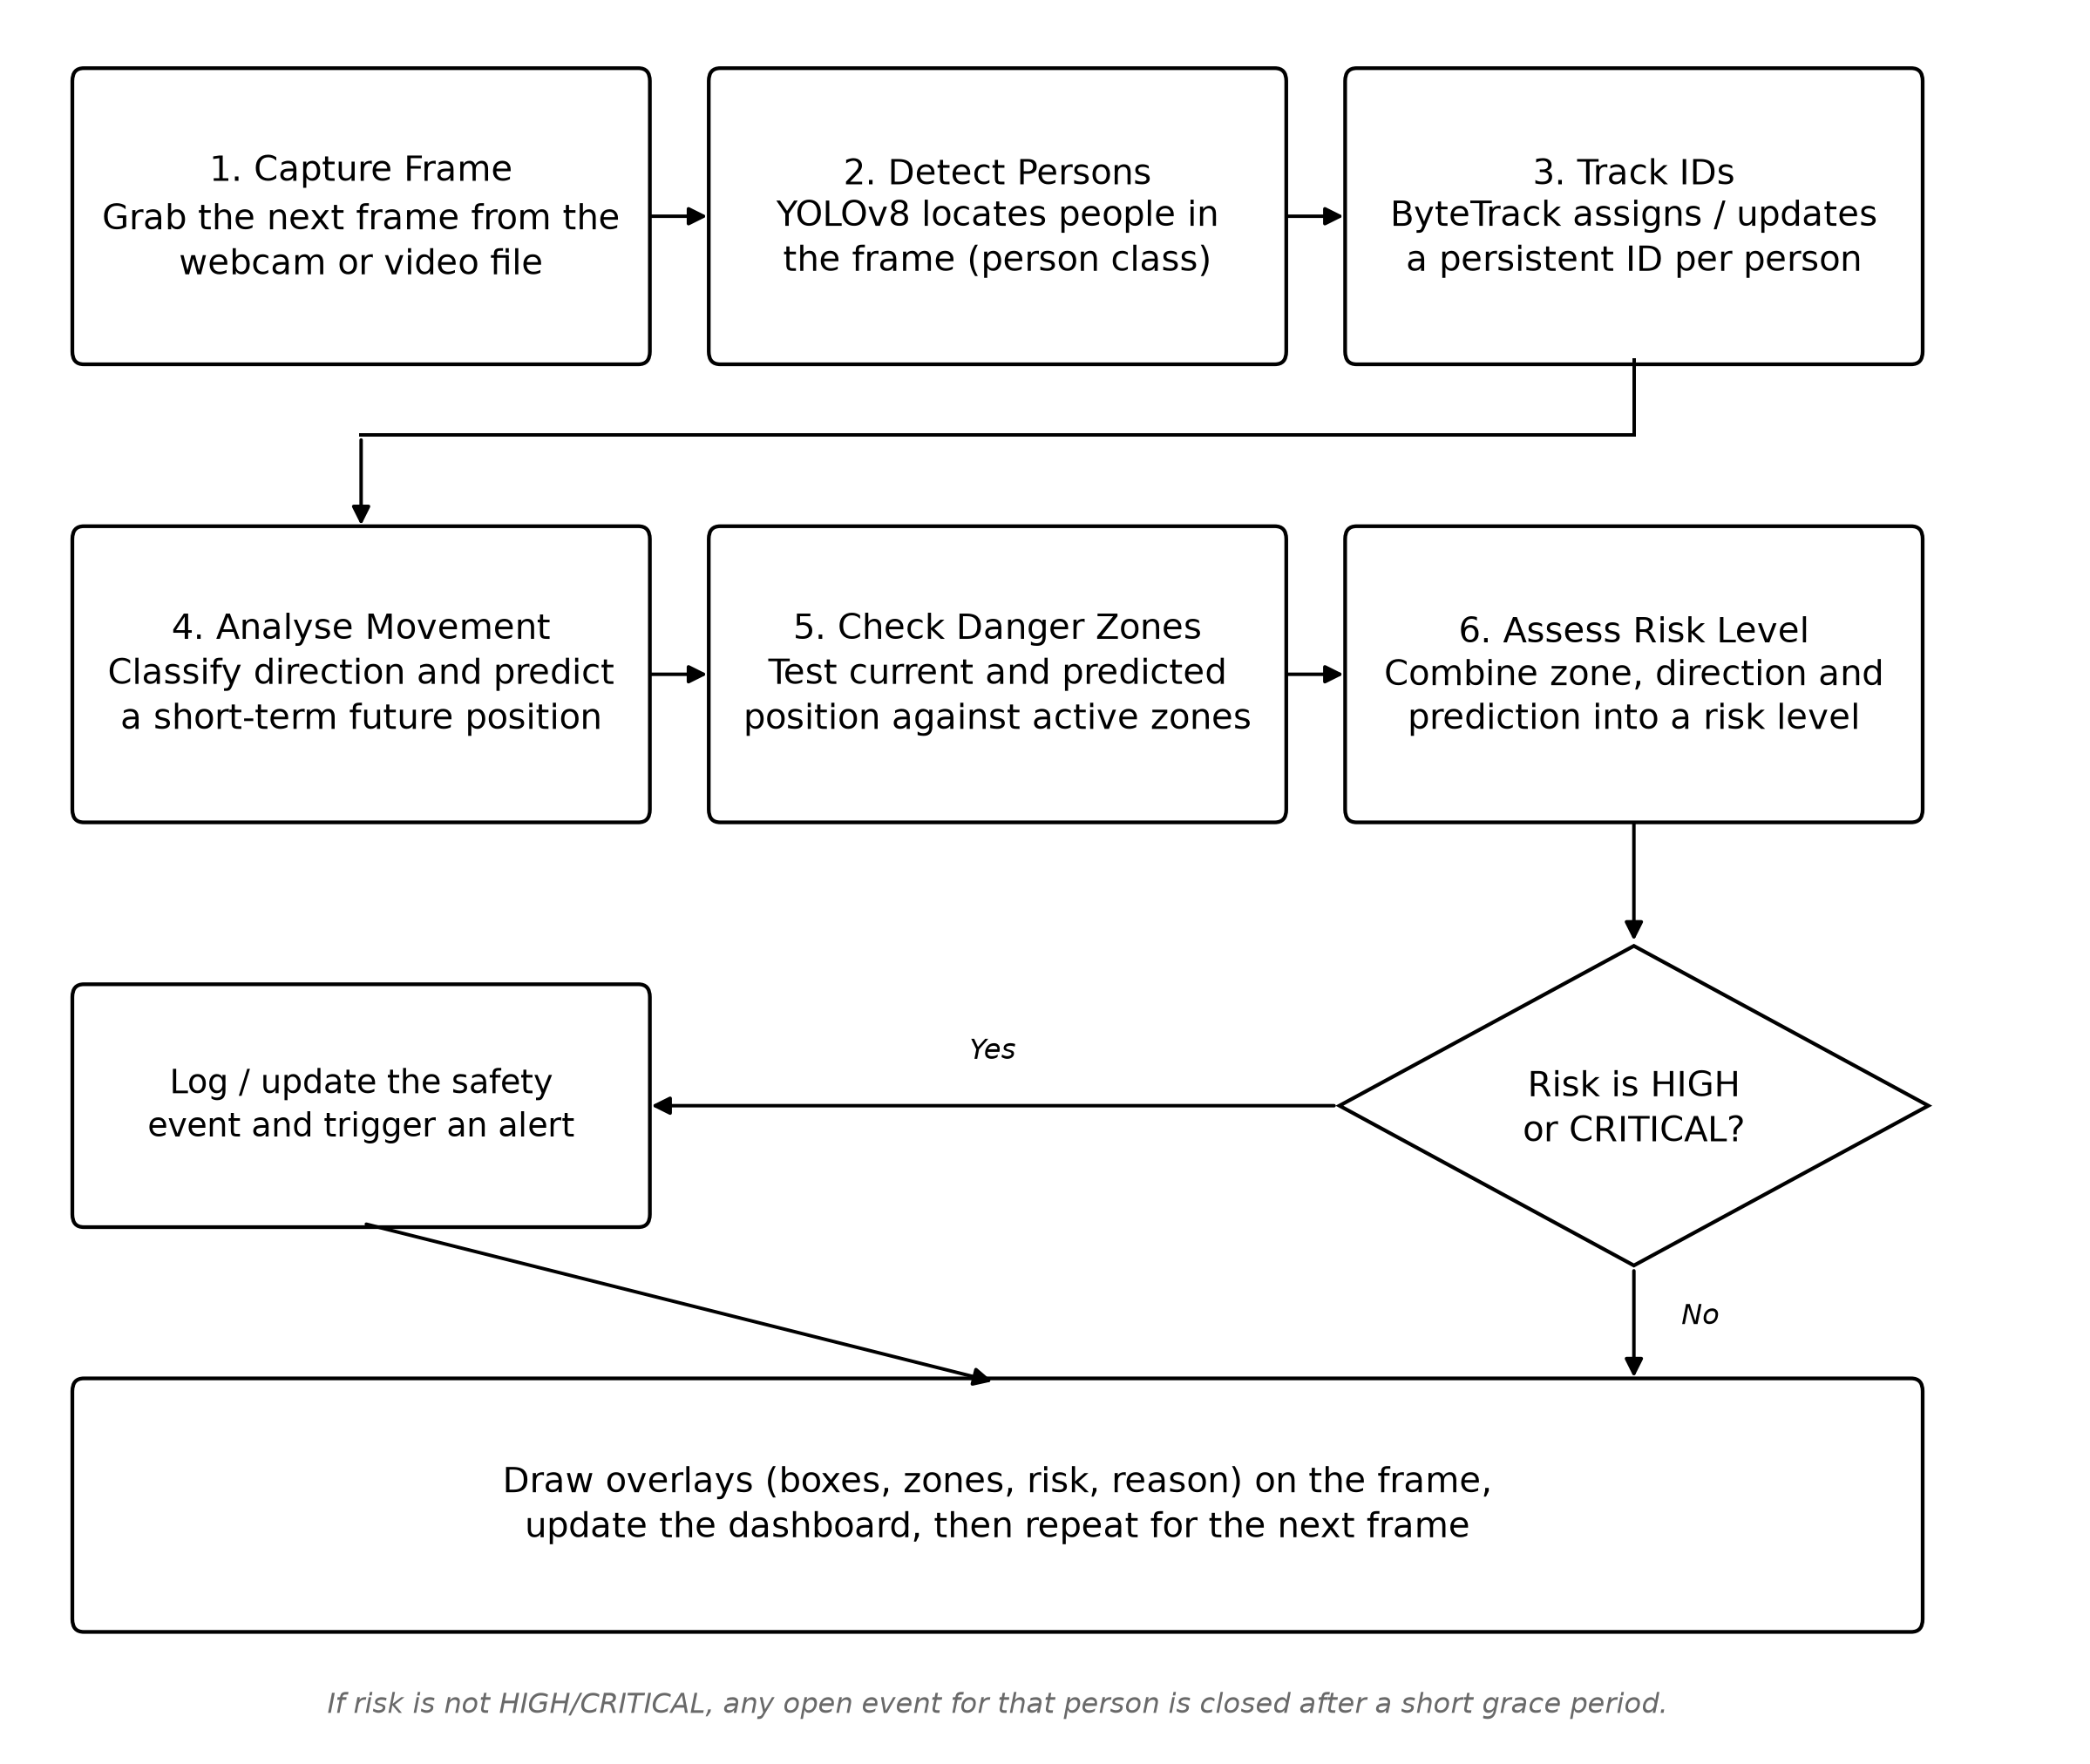
\includegraphics[width=5.9in]{images/fig_3_1_flowchart.png}
\caption{Flowchart of the per-frame detection, tracking and risk-assessment algorithm}
\label{fig:3.1}
\end{figure}

\section{Risk-Assessment Algorithm}
For every tracked person in a frame, the algorithm performs the following steps:
\begin{enumerate}[leftmargin=*,itemsep=2pt]
\item Update the person's recent position history with their current centre position and bounding-box height.
\item Classify their movement direction from the smoothed change in position and box size over the recent history.
\item Estimate a short-term future position by linearly extrapolating the recent average velocity, and determine whether that projected position would enter an active danger zone within a configured time horizon.
\item Determine current zone occupancy by testing the person's position against each active danger-zone polygon.
\item Combine zone occupancy, movement direction and predicted zone entry, using a fixed rule table, into a target risk level; escalate to that level immediately if it is higher than the current level, but only de-escalate to a lower level after it has been requested for several consecutive frames, to avoid flicker.
\item Build a plain-language explanation of the decision from the same inputs used to compute it.
\item If the resulting risk level is HIGH or CRITICAL, open or extend a safety event for that person in the event log, recording the zone, direction, explanation and frame range; otherwise, close any open event for that person after a short grace period.
\end{enumerate}

\section{Performance Metrics}
The performance of the prototype was measured directly, without requiring any ground truth, by running the full detection--tracking--risk pipeline over 90 consecutive live webcam frames on a standard laptop CPU, with no GPU. The measured values are given in Table 3.1.

\begin{table}[H]
\centering
\begin{tabular}{|p{3.4in}|p{2.0in}|}
\hline
\textbf{Metric} & \textbf{Measured value} \\ \hline
Average frames per second & 8.61 \\ \hline
Minimum / maximum FPS & 0.51 / 13.43 \\ \hline
Average per-frame processing time & 148.8 ms \\ \hline
95th-percentile per-frame processing time & 205.7 ms \\ \hline
Peak memory usage & 413.1 MB \\ \hline
\end{tabular}
\caption{Performance metrics (measured)}
\label{tab:3.1}
\end{table}

These figures confirm that the full pipeline, including detection, tracking, zone checking, risk assessment and dashboard rendering, runs in real time on ordinary laptop hardware without a dedicated GPU. Detection accuracy, tracking identity consistency and predictive-alert accuracy were not evaluated against annotated ground truth in this phase of the project, since no suitably annotated vehicle blind-spot footage was available; this is identified as future work in Chapter 5.

\section{Implementation Plan}
The implementation followed an incremental sequence, so that a working subset of the system was available for testing at each stage:
\begin{itemize}[leftmargin=*,itemsep=2pt]
\item Stage 1 -- Core detection: YOLOv8-based person detection, replacing an earlier age-classification heuristic that was found to be unreliable.
\item Stage 2 -- Tracking and zones: persistent tracking with ByteTrack, replacement of the single static region with configurable polygon danger zones, and a first explainable risk engine based on zone occupancy and movement direction.
\item Stage 3 -- Prediction and events: short-term trajectory prediction, predictive zone-conflict detection, and a safety-event state machine persisted to a SQLite database.
\item Stage 4 -- Dashboard: a Streamlit dashboard with live monitoring, a predictive-safety panel, a visual zone editor, incident analytics and a scenario simulator for recorded video, all built on the same underlying pipeline.
\item Stage 5 -- Evaluation and testing: an evaluation module for detection, tracking, predictive and performance metrics, and an automated test suite covering the zone geometry, risk engine, trajectory prediction and event-logging logic.
\end{itemize}

% ======================================================================
\chapter{RESULTS}

\section{Live Monitoring -- High-Risk Detection}
Fig no 4.1 shows the Live Monitoring tab of the dashboard while a person is tracked approaching the FRONT danger zone. The system assigns the tracking ID PERSON \#01, classifies the current movement as CROSSING, and raises the overall risk to HIGH, shown in the on-screen overlay together with the FPS, the number of people currently inside the danger zone, and the danger-zone boundary.

\begin{figure}[H]
\centering
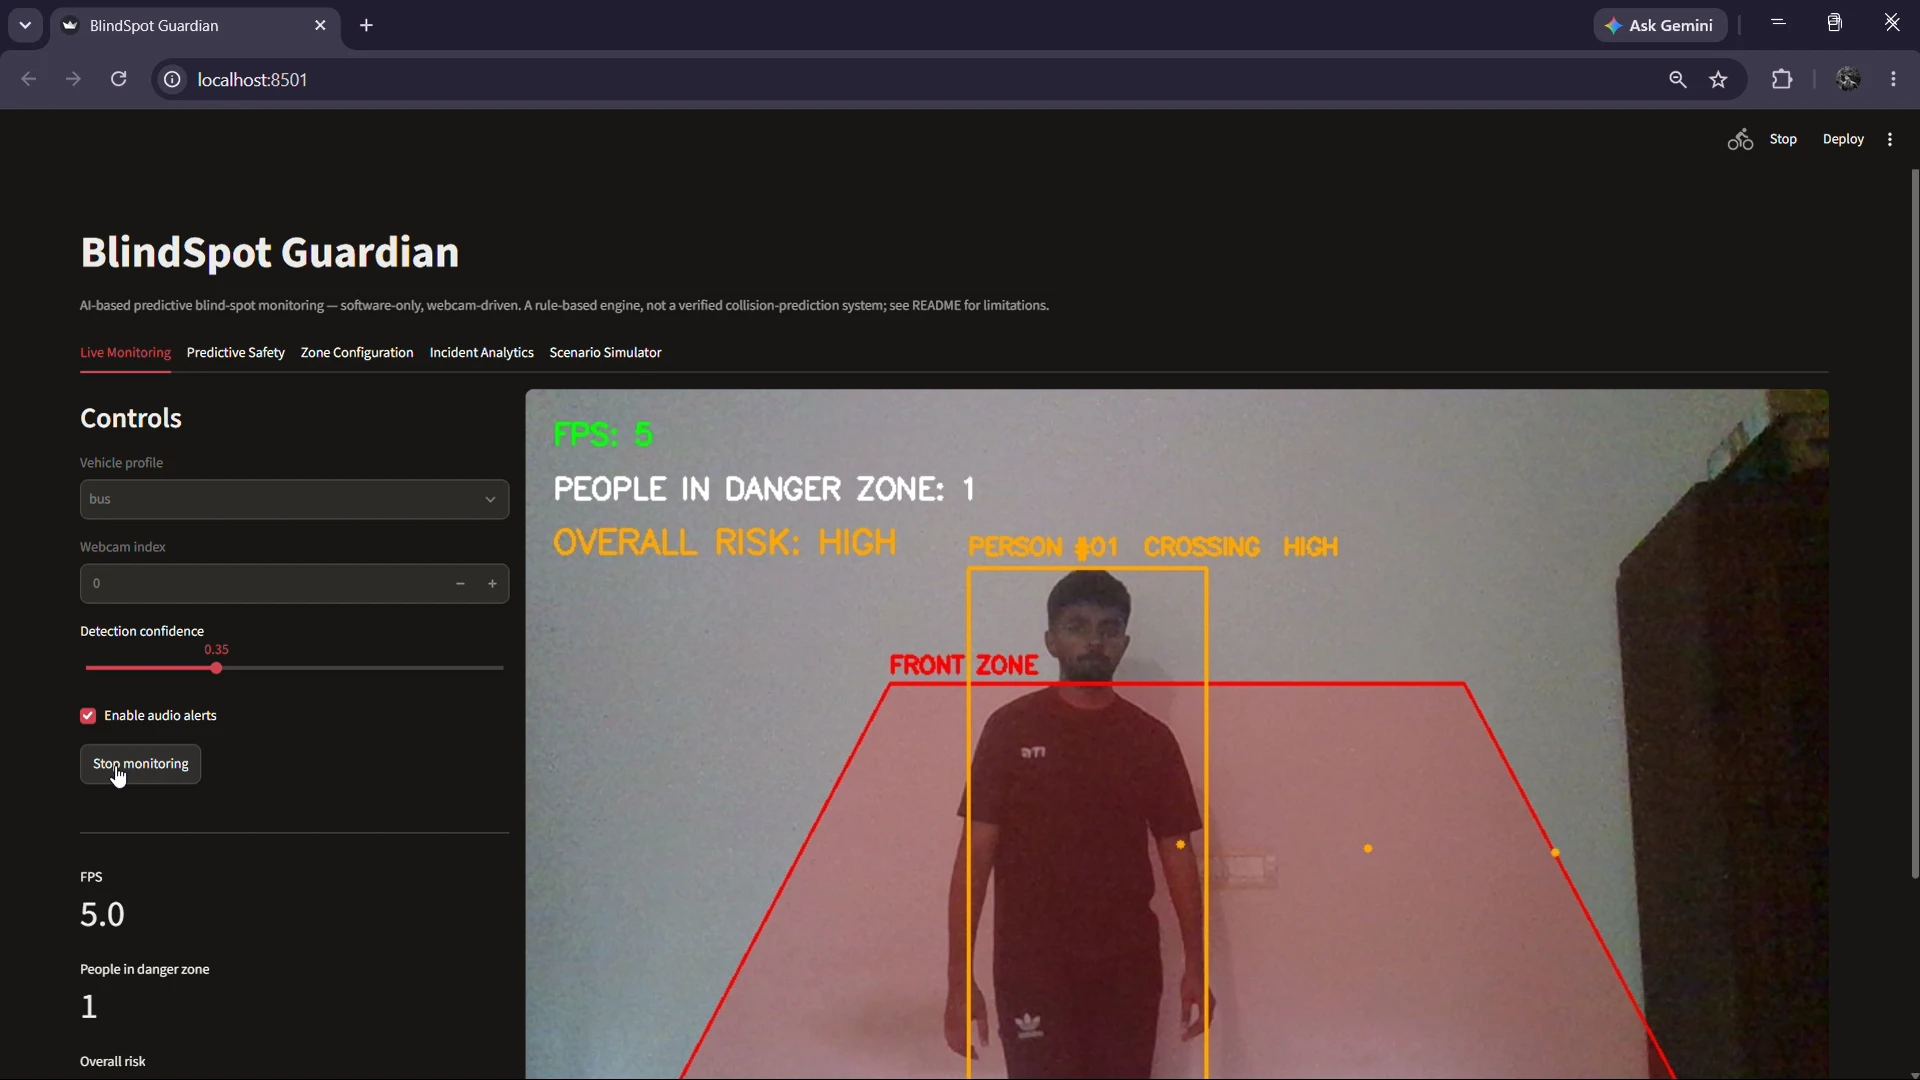
\includegraphics[width=4.6in]{images/live_high_risk.png}
\caption{Live Monitoring -- person approaching the danger zone (HIGH risk)}
\label{fig:4.1}
\end{figure}

\section{Live Monitoring -- Safe Condition}
Fig no 4.2 shows the same tab with the tracked person stationary and outside the FRONT danger zone. The overall risk correctly returns to SAFE, and the ``people in danger zone'' count returns to zero, demonstrating that the system distinguishes between hazardous and non-hazardous situations for the same tracked individual.

\begin{figure}[H]
\centering
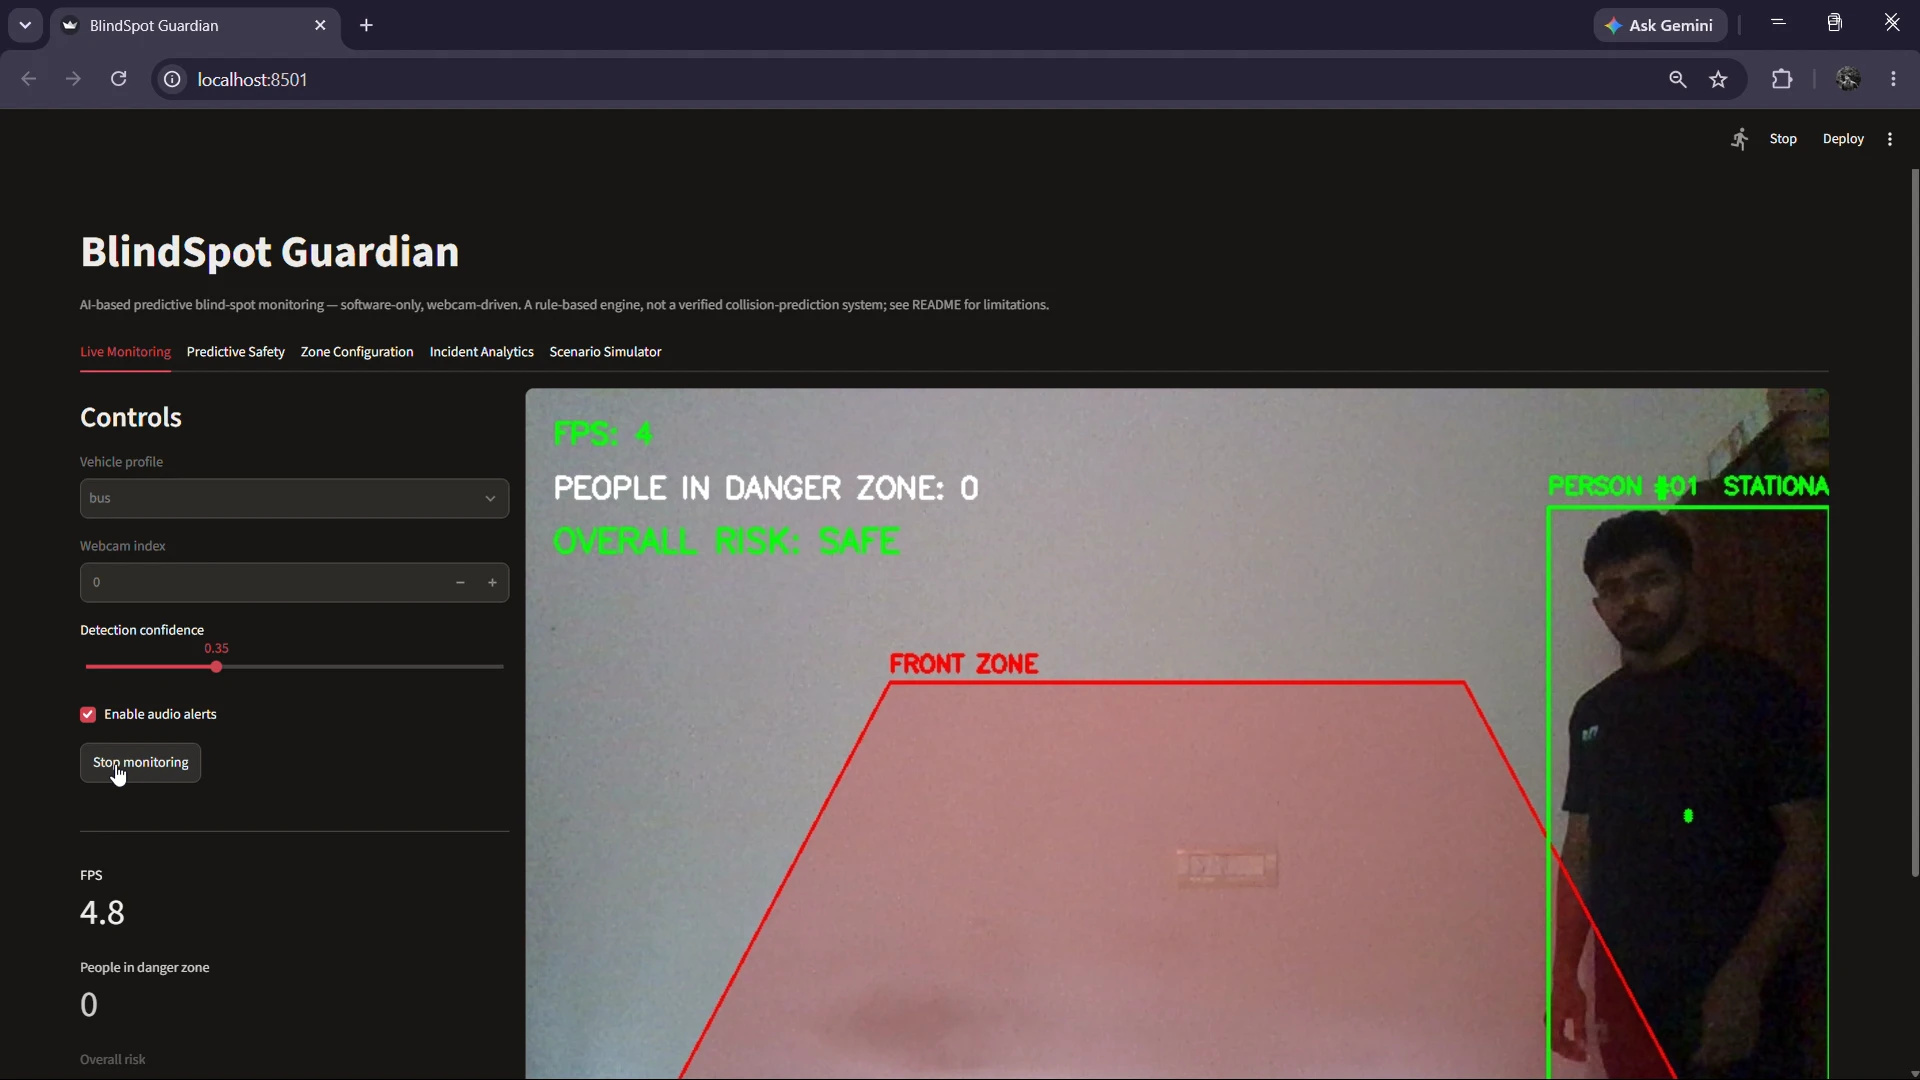
\includegraphics[width=4.6in]{images/live_safe.png}
\caption{Live Monitoring -- stationary person outside the danger zone (SAFE)}
\label{fig:4.2}
\end{figure}

\section{Zone Configuration}
Fig no 4.3 shows the Zone Configuration tab, where the FRONT danger zone of the bus profile is displayed as an editable polygon overlaid on the live camera preview. Zone corner points can be placed directly on the image, and the resulting polygon, stored as frame-fraction coordinates, is saved back into the vehicle-profile configuration.

\begin{figure}[H]
\centering
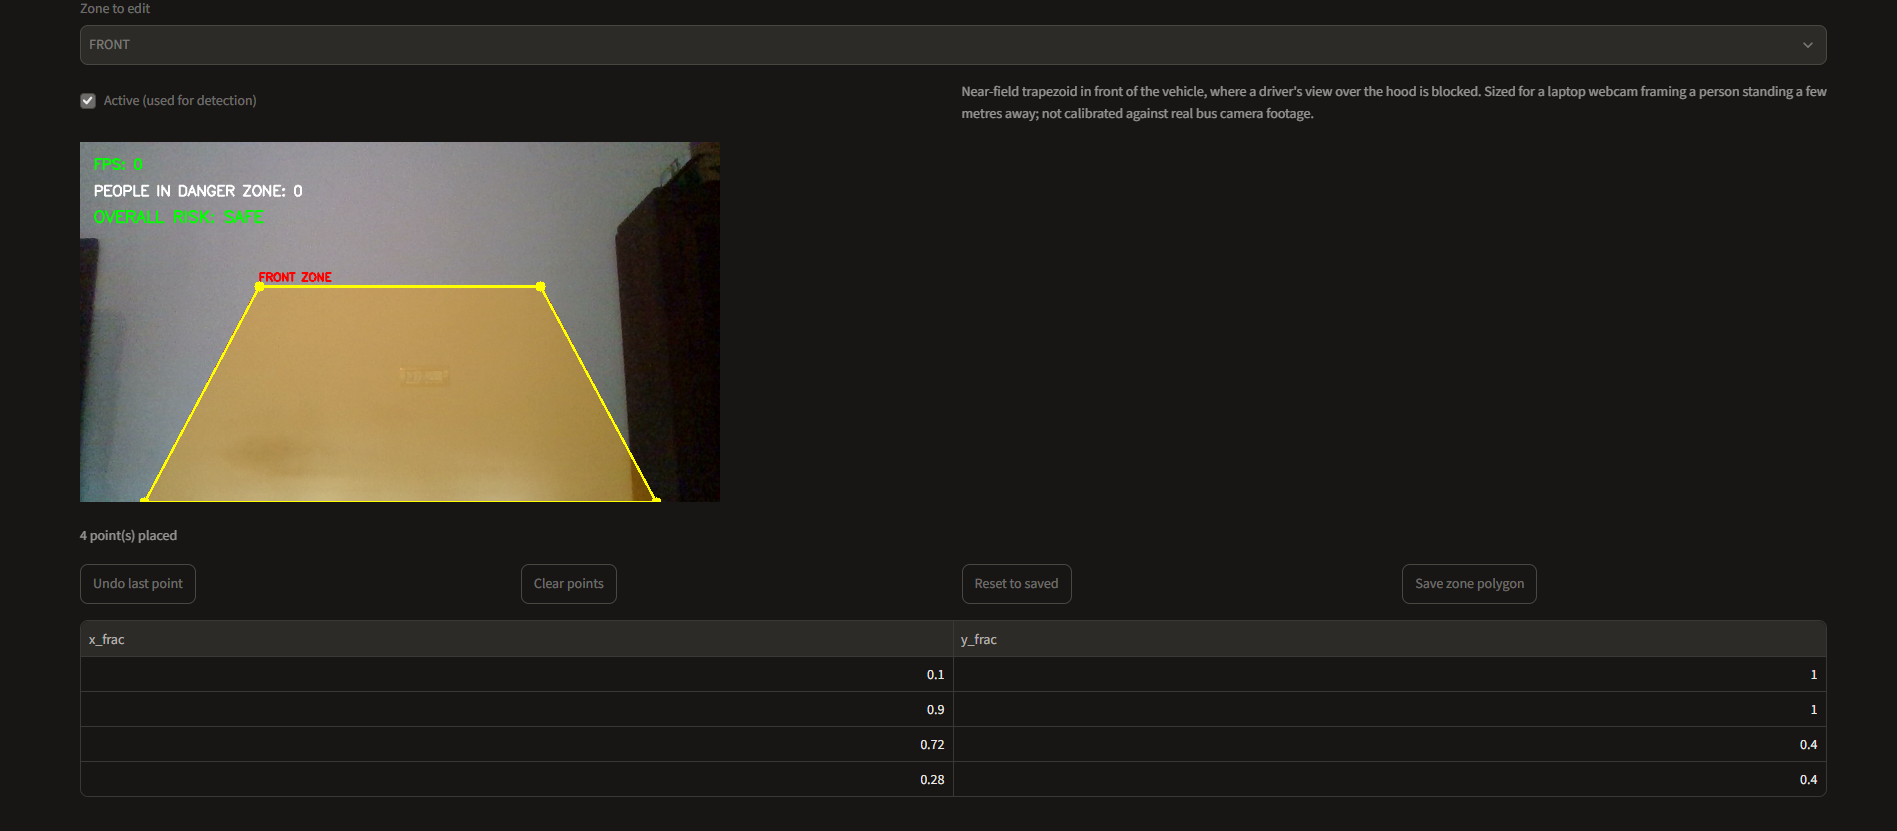
\includegraphics[width=5.6in]{images/zone_config.png}
\caption{Zone Configuration -- danger-zone editor with live camera preview}
\label{fig:4.3}
\end{figure}

\section{Incident Analytics -- Event Statistics}
Fig no 4.4 shows the Incident Analytics tab's summary charts, computed from the actual safety events logged by the system: a bar chart of events by risk level (HIGH and CRITICAL) and a pie chart of events by zone, including events that were opened from a predicted rather than an actual zone entry, labelled ``FRONT (predicted)'' to keep the two cases distinct.

\begin{figure}[H]
\centering
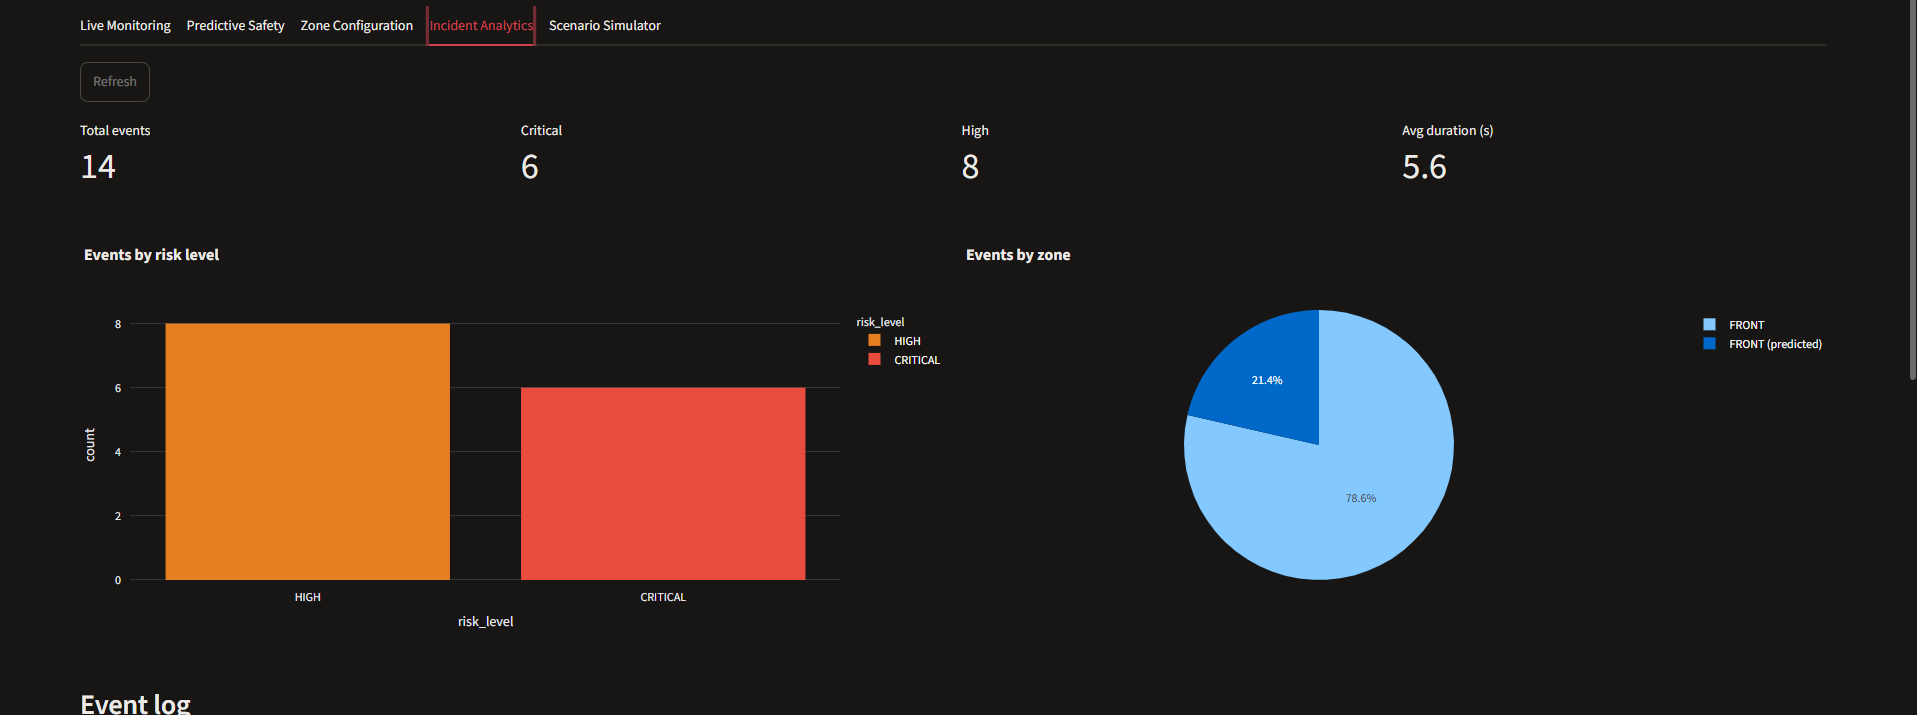
\includegraphics[width=5.6in]{images/analytics_charts.png}
\caption{Incident Analytics -- event statistics by risk level and zone}
\label{fig:4.4}
\end{figure}

\section{Incident Analytics -- Event Log}
Fig no 4.5 shows the corresponding event log table, listing each logged safety event with its tracking ID, zone, risk level, event type, movement direction, explanation, source, start and end time, and frame range, confirming that one continuous encounter is recorded as a single event rather than one row per frame.

\begin{figure}[H]
\centering
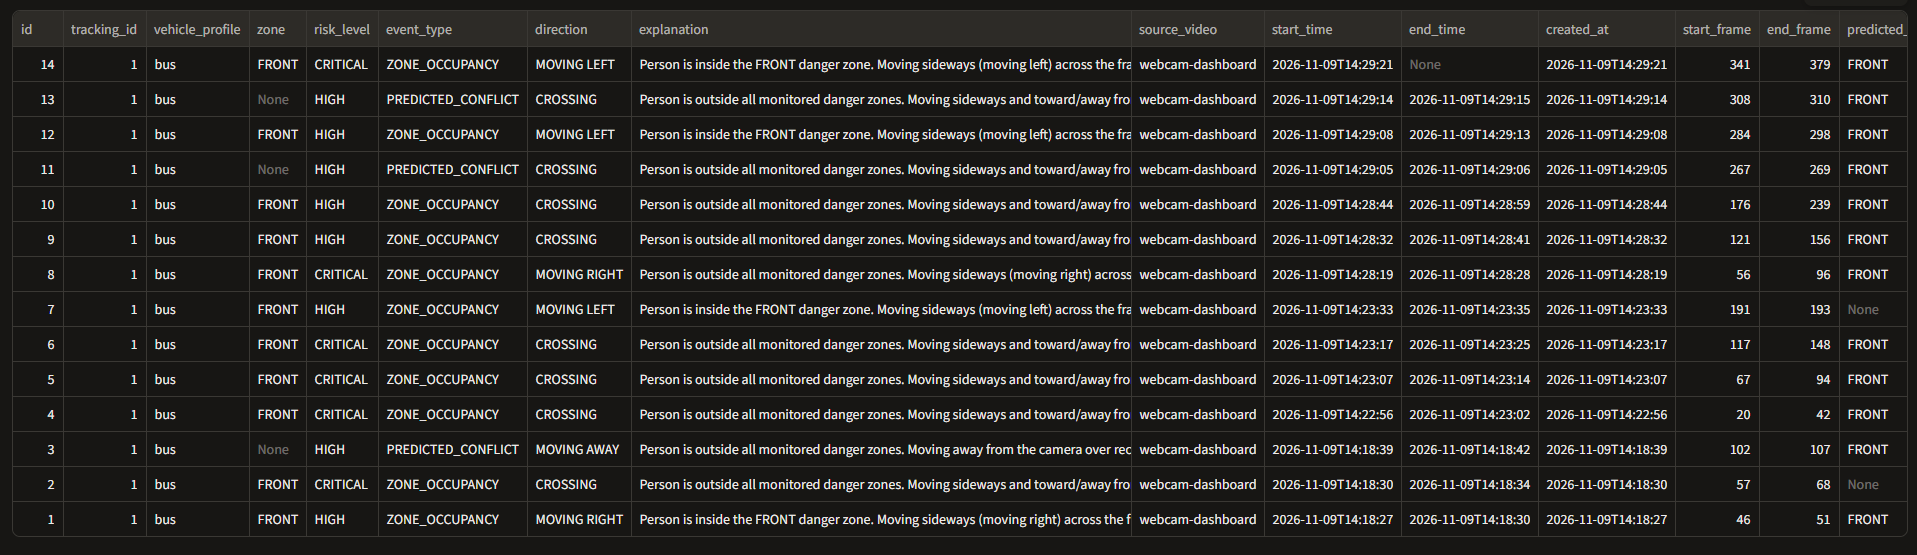
\includegraphics[width=5.6in]{images/analytics_table.png}
\caption{Incident Analytics -- safety event log}
\label{fig:4.5}
\end{figure}

% ======================================================================
\chapter{CONCLUSION}

\section{Conclusion}
An AI-based, software-only vehicle blind-spot monitoring system has been designed and implemented. The prototype detects people using YOLOv8, assigns them persistent identities using ByteTrack, analyses their movement direction, estimates their short-term trajectory, checks their position and predicted path against configurable danger zones, and assigns an explainable, dynamic risk level supported by a plain-language reason. Safety-relevant events are logged automatically, and all of this is presented through an interactive Streamlit dashboard with live monitoring, predictive-safety detail, a visual zone editor, incident analytics and a scenario simulator.

The work addresses the gap identified in Chapter 1, where the earlier baseline system could detect people but could not track them persistently, analyse their movement, predict likely zone entries, or explain its own risk decisions. On a standard laptop with no GPU, the complete pipeline, including detection, tracking, zone checking, risk assessment and dashboard rendering, sustains an average of 8.61 frames per second, confirming that the approach is practical on ordinary computing hardware.

\section{Key Outcomes}
\begin{itemize}[leftmargin=*,itemsep=2pt]
\item Persistent multi-person tracking with ByteTrack, giving each detected person a stable identity across frames instead of independent per-frame detections.
\item Movement-direction analysis and short-term trajectory prediction, including predictive zone-conflict detection that can raise risk before a person actually enters a danger zone.
\item A configurable, polygon-based danger-zone system supporting multiple named zones per vehicle profile.
\item A rule-based, explainable risk-assessment engine with temporal hysteresis and a plain-language reason attached to every decision.
\item Automatic safety-event logging to a database, with one row per continuous encounter rather than per frame, and incident replay for events whose source video is still available.
\item A five-tab Streamlit dashboard (Live Monitoring, Predictive Safety, Zone Configuration, Incident Analytics, Scenario Simulator) built on one shared pipeline implementation.
\item An evaluation module and an automated test suite (45 tests) covering the zone geometry, risk engine, trajectory prediction, event logging and the evaluation logic itself.
\end{itemize}

\section{Limitations and Future Scope}
The current system is software-only and has been demonstrated using a laptop webcam and prerecorded video; it does not yet control real vehicle hardware such as brakes or warning lights, and the danger-zone geometry used is sized for webcam demonstration rather than calibrated against real bus camera footage. Trajectory prediction uses a simple linear extrapolation rather than a learned motion model, and detection, tracking and predictive-alert accuracy have not yet been evaluated against annotated ground-truth footage, since no suitably annotated vehicle blind-spot dataset was available during this phase.

The following enhancements are identified for future work:
\begin{itemize}[leftmargin=*,itemsep=2pt]
\item Calibrating danger-zone geometry against real bus-mounted camera footage.
\item Evaluating detection precision/recall, tracking identity consistency and predictive-alert accuracy against annotated ground-truth video, for which the evaluation tooling has already been built.
\item Multi-camera integration, so that all four sides of a vehicle can be monitored simultaneously rather than one active zone at a time.
\item Improved trajectory prediction using a learned motion model and larger pedestrian-trajectory datasets.
\item Edge deployment on low-power, vehicle-mountable hardware, and optional integration with real hardware alerts.
\item Testing across a wider range of traffic, lighting and vehicle configurations.
\end{itemize}

\begin{samepage}
\section{SDG Alignment}
The project supports three UN Sustainable Development Goals (Table 5.1).

\begin{table}[H]
\centering
\begin{tabular}{|p{0.7in}|p{1.6in}|p{3.0in}|}
\hline
\textbf{SDG} & \textbf{Goal} & \textbf{Contribution of the project} \\ \hline
SDG 3 & Good Health and Well-Being & Aims to reduce pedestrian injuries and fatalities around large vehicles through earlier, more informed blind-spot awareness. \\ \hline
SDG 9 & Industry, Innovation and Infrastructure & Applies modern AI-based computer-vision techniques (detection, tracking, trajectory prediction) to vehicle safety in a software-only, accessible form. \\ \hline
SDG 11 & Sustainable Cities and Communities & Supports safer road and public-transport environments, particularly around school buses and public-transport vehicles in urban and semi-urban settings. \\ \hline
\end{tabular}
\caption{Alignment of the project with the UN Sustainable Development Goals}
\label{tab:5.1}
\end{table}
\end{samepage}

% ======================================================================
\begin{thebibliography}{9}

\bibitem{redmon2016}
J.\ Redmon, S.\ Divvala, R.\ Girshick, and A.\ Farhadi, ``You only look once: Unified, real-time object detection,'' in \textit{Proc.\ IEEE Conf.\ Comput.\ Vis.\ Pattern Recognit.\ (CVPR)}, 2016, pp.\ 779--788, doi: 10.1109/CVPR.2016.91.

\bibitem{bewley2016}
A.\ Bewley, Z.\ Ge, L.\ Ott, F.\ Ramos, and B.\ Upcroft, ``Simple online and realtime tracking,'' in \textit{Proc.\ IEEE Int.\ Conf.\ Image Process.\ (ICIP)}, 2016, pp.\ 3464--3468, doi: 10.1109/ICIP.2016.7533003.

\bibitem{zhang2022}
Y.\ Zhang et al., ``ByteTrack: Multi-object tracking by associating every detection box,'' in \textit{Proc.\ Eur.\ Conf.\ Comput.\ Vis.\ (ECCV)}, 2022, doi: 10.1007/978-3-031-20047-2\_1.

\bibitem{alahi2016}
A.\ Alahi et al., ``Social LSTM: Human trajectory prediction in crowded spaces,'' in \textit{Proc.\ IEEE Conf.\ Comput.\ Vis.\ Pattern Recognit.\ (CVPR)}, 2016, pp.\ 961--971, doi: 10.1109/CVPR.2016.110.

\bibitem{gunning2019}
D.\ Gunning and D.\ W.\ Aha, ``DARPA's explainable artificial intelligence (XAI) program,'' \textit{AI Magazine}, vol.\ 40, no.\ 2, pp.\ 44--58, 2019, doi: 10.1609/aimag.v40i2.2850.

\bibitem{jocher2023}
G.\ Jocher, A.\ Chaurasia, and J.\ Qiu, ``Ultralytics YOLO (YOLOv8),'' software, version 8.0.0, 2023. [Online]. Available: \url{https://github.com/ultralytics/ultralytics}

\bibitem{lee2023}
H.\ Lee, H.\ Cho, B.\ Noh, and H.\ Yeo, ``NAVIBox: Real-Time Vehicle--Pedestrian Risk Prediction System in an Edge Vision Environment,'' \textit{Electronics}, vol.\ 12, no.\ 20, Art.\ no.\ 4311, 2023, doi: 10.3390/electronics12204311.

\end{thebibliography}

\end{document}
